\documentclass[conference,onecolumn]{IEEEtran}
\usepackage{hyperref}
\usepackage[utf8]{inputenc}
\usepackage[french]{babel}
\usepackage{amsmath,amssymb,amsfonts}
\usepackage{algorithmic}
\usepackage{graphicx}
\usepackage{textcomp}
\usepackage{xcolor}
\usepackage{lipsum, babel}
\def\BibTeX{{\rm B\kern-.05em{\sc i\kern-.025em b}\kern-.08em
    T\kern-.1667em\lower.7ex\hbox{E}\kern-.125emX}}
\begin{document}

\title{Atténuation du bruit dans des signaux audios a travers l’implémentation de méthodes classiques et une méthode hybride\\
}

\author{\IEEEauthorblockN{1\textsuperscript{st} José Miguel Galindo Barco}
\IEEEauthorblockA{\textit{Ecole d’ingénieurs}\\
\textit{Génie de systèmes} \\
\textit{Université EAFIT}\\
\href{mailto:jmgalindob@eafit.edu.co}{jmgalindob@eafit.edu.co}
}
\and
\IEEEauthorblockN{2\textsuperscript{nd} Juan José Tamayo Acevedo}
\IEEEauthorblockA{\textit{Ecole de sciences}\\
\textit{Génie mathématique} \\
\textit{Université EAFIT}\\
\href{mailto:jjtamayoa@eafit.edu.co}{jjtamayoa@eafit.edu.co}
}
\and
\IEEEauthorblockN{3\textsuperscript{rd} Salomón Cardeño Luján}
\IEEEauthorblockA{\textit{Ecole de sciences}\\
\textit{Génie mathématique} \\
\textit{Université EAFIT}\\
\href{mailto:scardenol@eafit.edu.co}{scardenol@eafit.edu.co}
}
}

\maketitle

\begin{abstract}
%\lipsum[3]
\end{abstract}

\section{Introduction}
%\lipsum[1]

\section{Concepts fondamentaux}
Signal: un signal est la representation physique de l'information, qu'il convoit de sa source a sa destination.

Bruit: Un bruit correspond a tout phénomène gênant la transmission ou l'interpretation d'un signal


\subsection{Signal sonore et note audio}
%\lipsum[3]

\subsection{Représentation d’un fichier audio dans un ordinateur}
%\lipsum[3]

\subsection{Bruit et types de bruit}
%\lipsum[3]

\section{Méthodes}
Le but de ce projet est de implementer le filtrage dans les notes audios dans l'objectif d'attenuer le bruit present. Pour cela nous allons implementé le filtrage analogique avec une approximation de Butterworth, la méthode RNN et un autre qui reste définir.

\section{Résultats et comparaison des méthodes}

\begin{figure}[htp]
    \centering
    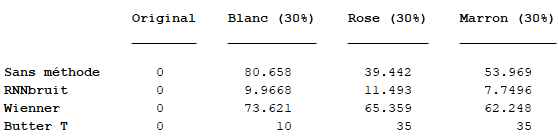
\includegraphics[width=15cm]{Tabla.png}
    \caption{Résultats des méthodes pour 30\% du bruit blanc, rose et marron.}
    \label{fig:Résultats}
\end{figure}

En étudiant les résultats obtenus par l'implémentation du filtre passe-bas avec une approximation de Butter Worth, nous confirmant les hypothèses théoriques vues précédemment. En effet, compte tenu que l’approximation de Butter Worth permet d’avoir une précision en amplitude. Cette précision est centre sur des bases fréquences. Nous voyons cela évidence dans le filtrage des bruits ajouter à notre signal. Lorsque nous ajoutons du bruit blanc et nous filtrons le signal résultant, nous constatons une diminution du pourcentage du bruit présent dans le signal. Alors que lorsque nous effectuons le même procédé pour le bruit rose et le bruit marron, le pourcentage de bruit ne change pas. Donc cette méthode avec cette approximation particulière est bien plus convenable pour filtrer le bruit blanc présent dans les enregistrements audios.

Dans le cas de la méthode hybride du RNNbruit, nous observons que cette méthode est belle et bien convenable pour les différents types de bruit additionnés. En effet, nous constatons une atténuation du bruit considérable dans chacun des cas. De plus, nous remarquons que cette méthode ne gêne pas la transmission du signal sonore, en d'autre thermes cette méthode lise et "purifie" le signal orignal. Nous pouvons expliquer ce comportement par la nature adaptative de la méthode, dû au fait de l'implémentation de réseau de neurones récurrents pour faire face au bruit non harmonique. Cependant, la partie traditionnelle de cette méthode dite hybride se charge du bruit harmonique comme nous l'avant vue précédemment dans la partie théorique.


\end{document}

